%%\documentclass[a4paper,12pt,oneside]{llncs}
\documentclass[12pt,letterpaper]{article}
\usepackage[right=2cm,left=3cm,top=2cm,bottom=2cm,headsep=0cm]{geometry}

%%%%%%%%%%%%%%%%%%%%%%%%%%%%%%%%%%%%%%%%%%%%%%%%%%%%%%%%%%%
%% Juego de caracteres usado en el archivo fuente: UTF-8
\usepackage{ucs}
\usepackage[utf8x]{inputenc}

%%%%%%%%%%%%%%%%%%%%%%%%%%%%%%%%%%%%%%%%%%%%%%%%%%%%%%%%%%%
%% Juego de caracteres usado en la salida dvi
%% Otra posibilidad: \usepackage{t1enc}
\usepackage[T1]{fontenc}

%%%%%%%%%%%%%%%%%%%%%%%%%%%%%%%%%%%%%%%%%%%%%%%%%%%%%%%%%%%
%% Ajusta maergenes para a4
%\usepackage{a4wide}

%%%%%%%%%%%%%%%%%%%%%%%%%%%%%%%%%%%%%%%%%%%%%%%%%%%%%%%%%%%
%% Uso fuente postscript times, para que los ps y pdf queden y pequeños...
\usepackage{times}

%%%%%%%%%%%%%%%%%%%%%%%%%%%%%%%%%%%%%%%%%%%%%%%%%%%%%%%%%%%
%% Posibilidad de hipertexto (especialmente en pdf)
%\usepackage{hyperref}
\usepackage[bookmarks = true, colorlinks=true, linkcolor = black, citecolor = black, menucolor = black, urlcolor = black]{hyperref}

%%%%%%%%%%%%%%%%%%%%%%%%%%%%%%%%%%%%%%%%%%%%%%%%%%%%%%%%%%%
%% Graficos 
\usepackage{graphics,graphicx}

%%%%%%%%%%%%%%%%%%%%%%%%%%%%%%%%%%%%%%%%%%%%%%%%%%%%%%%%%%%
%% Ciertos caracteres "raros"...
\usepackage{latexsym}

%%%%%%%%%%%%%%%%%%%%%%%%%%%%%%%%%%%%%%%%%%%%%%%%%%%%%%%%%%%
%% Matematicas aun más fuertes (american math dociety)
\usepackage{amsmath}

%%%%%%%%%%%%%%%%%%%%%%%%%%%%%%%%%%%%%%%%%%%%%%%%%%%%%%%%%%%
\usepackage{multirow} % para las tablas
\usepackage[spanish,es-tabla]{babel}

%%%%%%%%%%%%%%%%%%%%%%%%%%%%%%%%%%%%%%%%%%%%%%%%%%%%%%%%%%%
%% Fuentes matematicas lo mas compatibles posibles con postscript (times)
%% (Esto no funciona para todos los simbolos pero reduce mucho el tamaño del
%% pdf si hay muchas matamaticas....
\usepackage{mathptm}

%%% VARIOS:
%\usepackage{slashbox}
\usepackage{verbatim}
\usepackage{array}
\usepackage{listings}
\usepackage{multirow}

%% MARCA DE AGUA
%% Este package de "draft copy" NO funciona con pdflatex
%%\usepackage{draftcopy}
%% Este package de "draft copy" SI funciona con pdflatex
%%%\usepackage{pdfdraftcopy}
%%%%%%%%%%%%%%%%%%%%%%%%%%%%%%%%%%%%%%%%%%%%%%%%%%%%%%%%%%%
%% Indenteacion en español...
\usepackage[spanish]{babel}

\usepackage{listingsutf8}
% Para escribir código en C
% \begin{lstlisting}[language=C]
% #include <stdio.h>
% int main(int argc, char* argv[]) {
% puts("Hola mundo!");
% }
% \end{lstlisting}


\title{Práctica 1}
\author{Jesús Rodríguez Heras\\
	Arantzazu Otal Alberro}

\begin{document}
	
	\maketitle
%	\begin{abstract} %Poner esto en todas las prácticas de PCTR
%%		\begin{center}
%%			\noindent
%			
%%		\end{center}
%	\end{abstract}
	\thispagestyle{empty}
	\newpage
	
%	\tableofcontents
%	\newpage
	
	%%\listoftables
	%%\newpage
	
	%%\listoffigures
	%%\newpage
	
	%%%% REAL WORK BEGINS HERE:
	
	%%Configuracion del paquete listings
	\lstset{language=bash, numbers=left, numberstyle=\tiny, numbersep=10pt, firstnumber=1, stepnumber=1, basicstyle=\small\ttfamily, tabsize=1, extendedchars=true, inputencoding=utf8/latin1, breaklines=true}
	
\section{Instalación de máquinas virtuales mediante Vagrant}
\begin{enumerate}
	\item \textbf{Crear una máquina virtual usando Vagrant.} \\
	Para descargar la máquina virtual usamos \texttt{vagrant init hashicorp/precise64} y para lanzarla \texttt{vagran up}.
	\item \textbf{Actualizar el listado de los paquetes.} \\
	Para actualizar el listado de paquetes usamos \texttt{sudo apt-get update}.
	\item \textbf{Instalar el Apache:} \\
	Para la instalación de apache \texttt{sudo apt-get install -y apache2}.
	\item \textbf{Redirigir el puerto 80 para accederse localmente.} \\
	Para redirigir el puerto 80\footnote{Cuidado con el puerto 80 porque nos puede salir un error en el que nos dice que debemos usar un puerto superior al 1024. Por lo tanto, usaremos el 8080 en el archivo \texttt{Vagrantfile}, quedando \texttt{... guest:80, host: 8080} en la línea 3 del código anteriormente mostrado.} lo indicamos en el archivo \texttt{Vagrantfile} de la siguiente forma:
	\begin{lstlisting}[language=Bash]
	Vagrant.configure("2") do |config|
	config.vm.box = "hashicorp/precise64"
	config.vm.network :forwarded_port, guest: 80, host: 80
	end
	\end{lstlisting}
	
	Para entrar en la máquina virtual usamos \texttt{vagrant ssh}.
	
	Para comprobar que funciona correctamente, buscamos la dirección \texttt{127.0.0.1:80}\footnote{\texttt{127.0.0.1:8080} en caso de que no nos haya dejado usar el puerto 80.} en nuestro navegador, y nos redirigirá a la página de Apache de la máquina virtual.
		
\end{enumerate}

\begin{figure}[h]
	\centering
	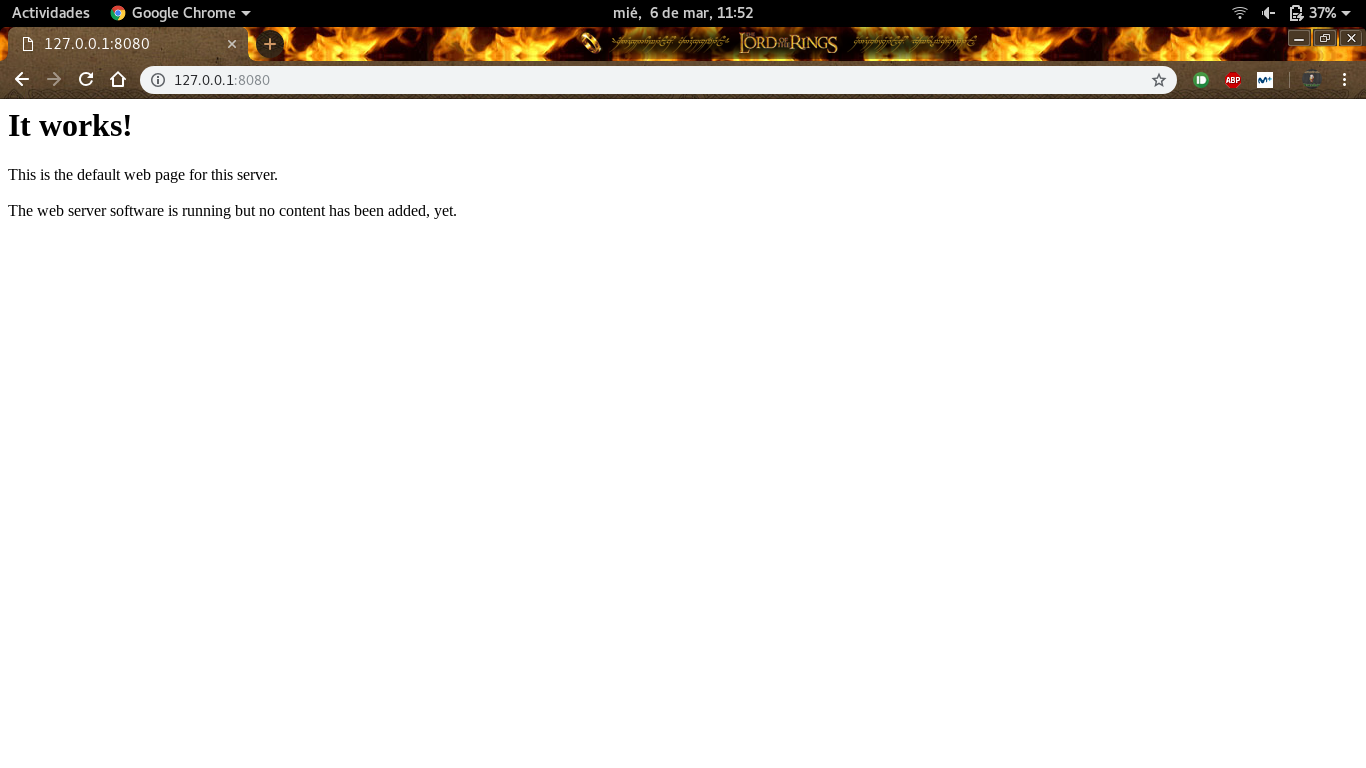
\includegraphics[scale=0.34]{apache.png}
\end{figure}

\section{Comandos básicos}
\begin{enumerate}
	\item \textbf{Mostrar todos los archivo txt del sistema.} \\ \texttt{find / -type f -name "*.txt"}
	\item \textbf{Modificar el ejercicio anterior para que no se muestren los errores de acceso.} \\ \texttt{find / -type f -name "*.txt" |\& grep -v "Permission denied"}
	\item \textbf{Mostrar el número de archivos txt del sistema.} \\ \texttt{find / -type f -name "*.txt" |\& grep -v "Permission denied" | wc -l}
	\item \textbf{Mostrar cuantos usuarios no pueden iniciar sesión} \\ \texttt{cat /etc/passwd | grep nologin | wc -l}
	\item \textbf{Mostrar el tipo de inicio de sesión de los usuarios que están dados de alta en el sistema, así como el número de cada uno de estos usuarios. La información se tiene que mostrar de forma ordenada por el número de usuarios.} \\ \texttt{cat /etc/passwd | cut -d : -f 7 | sort | uniq -c | sort -n}
\end{enumerate}

\section{Procesos}
\begin{enumerate}
	\item \textbf{Encuentra usando find y perm los programas con el setuid activado. ¿Cuáles son?} \\ 
	\texttt{find / -perm -4000 2>/dev/null}
	\item \textbf{Identificar los 3 procesos que se ejecutan con permisos de root que requieren más memoria.} \\
	\texttt{ps aux --sort -rss | grep ``root'' | head -n 3}
	\item \textbf{Monitorizar (con watch) la memoria libre. Deberá mostrarse cada 10 segundos la actual memoria libre (únicamente ese valor, sin ningún texto adicional).} \\
	\texttt{watch -n 10 'cat /proc/meminfo | grep "MemFree" | cut -d : -f 2'}
\end{enumerate}

\section{Gestión de usuarios}
\begin{enumerate}
	\item \textbf{Crear un usuario llamado con nuestras iniciales. El usuario tendrá home, bash y podrá iniciar sesión.}
	\texttt{sudo useradd -m -s /bin/bash JAROHA}
	\item \textbf{Crear un usuario llamado \textit{webuser} sin bash, ni home y que no pueda iniciar sesión.} \\
	\texttt{sudo useradd -M -s /bin/false webuser}
	\item \textbf{Crear un usuario llamado antonio que se pueda identificar como webuser (usando sudo) pero no como root.}
	\texttt{sudo useradd -m -s /bin/bash antonio} \\
	Luego, debemos cambiar en el archivo /etc/sudoers añadiendo al usuario antonio de la siguiente forma: \\
	\texttt{antonio ALL=(webuser) ALL}
\end{enumerate}

\section{/proc}
\begin{enumerate}
	\item \textbf{Identificar tres archivos y explicar su contenido.}
	\begin{itemize}
		\item \texttt{meminfo:} Nos muestra información de la memoria. Por ejemplo: memoria libre, memoria ocupada, etc.
		\item \texttt{version:} Nos muestra información sobre la versión del sistema.
		\item \texttt{partitions:} Nos muestra información a cerca de las particiones de nuestro sistema.
	\end{itemize}
	\item \textbf{Identificar al menos dos archivos que permitan escritura.} \\
	Con el comando \texttt{ls -l} podemos fijarnos en los permisos que tiene cada fichero. Dos ejemplos de archivos que permiten escritura son: \texttt{timer\_stats} y \texttt{mtrr}
\end{enumerate}

\section{Bash scripting}
\begin{enumerate}
	\item \textbf{Realizar un programa que permita cambiar el nombre de los archivos de un directorio dado como argumento de entrada. El nuevo nombre será un número secuencial, manteniendo la extensión.} 
	\lstinputlisting[language=Bash]{e1.sh}
	\item \textbf{Se pide realizar un programa que realice una copia de los directorios que cuelguen de /importante/ en media/backup, siguiendo las directivas:
	\begin{itemize}
		\item Cada directorio que cuelga de /importante/ deberá de guardarse en un fichero \texttt{.tgz}.
		\item Cada fichero de backup deberá de tener el nombre del directorio seguido de la fecha. La fecha estará en formato año, mes, día. Por ejemplo, para copiar el directorio \texttt{docencia} deberá tener el nombre \texttt{docencia\_20140404.tgz}.
	\end{itemize}}
	\lstinputlisting[language=Bash]{e2.sh}
	\item \textbf{Proponer una modificación al programa anterior, de tal modo de que parra cada directorio se guarden sólo los 5 últimos ficheros. Es decir, al copiar el sexto fichero asociado a un mismo directorio se borrará la copia más a ntigua.}
	\lstinputlisting[language=Bash]{e3.sh}
	\item \textbf{Utilizar el crontab para ejecutar el programa de backup cada día a las 5 de la mañana.} \\
	Para ejecutar el crontab usamos \texttt{crontab -e}.
		
	A continuación, seleccionamos el editor que más nos guste, en nuestro caso, \texttt{nano} (opción 2).
		
	Por último escribimos lo siguiente en el archivo de configuración de \texttt{crontab}:
	\begin{center}
		\texttt{0 5 * * * /home/vagrant/e3.sh}.
	\end{center}
		
	Al guardar, ya se queda activado y listo para ejecutarse a las 5 de la mañana.
\end{enumerate}
\end{document}